
\section{Sensor Setup}

\subsection{Light Curtain Basics}

\begin{figure}[h]
   \centering
   \begin{minipage}{0.5\textwidth}
       \centering
       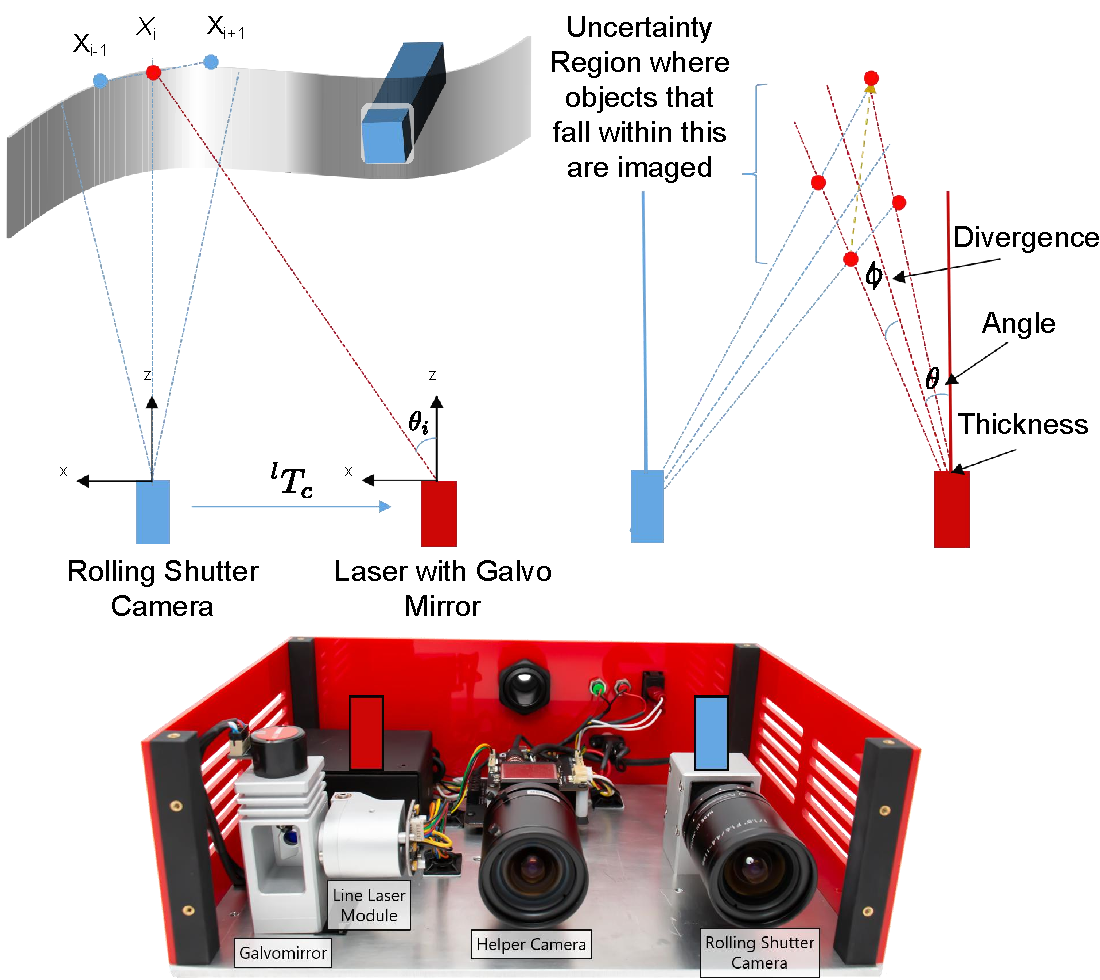
\includegraphics[width=1.0\textwidth]{figures/LC.pdf} % first figure itself
   \end{minipage}\hfill
   % \begin{minipage}{0.3\textwidth}
   %     \centering
   %     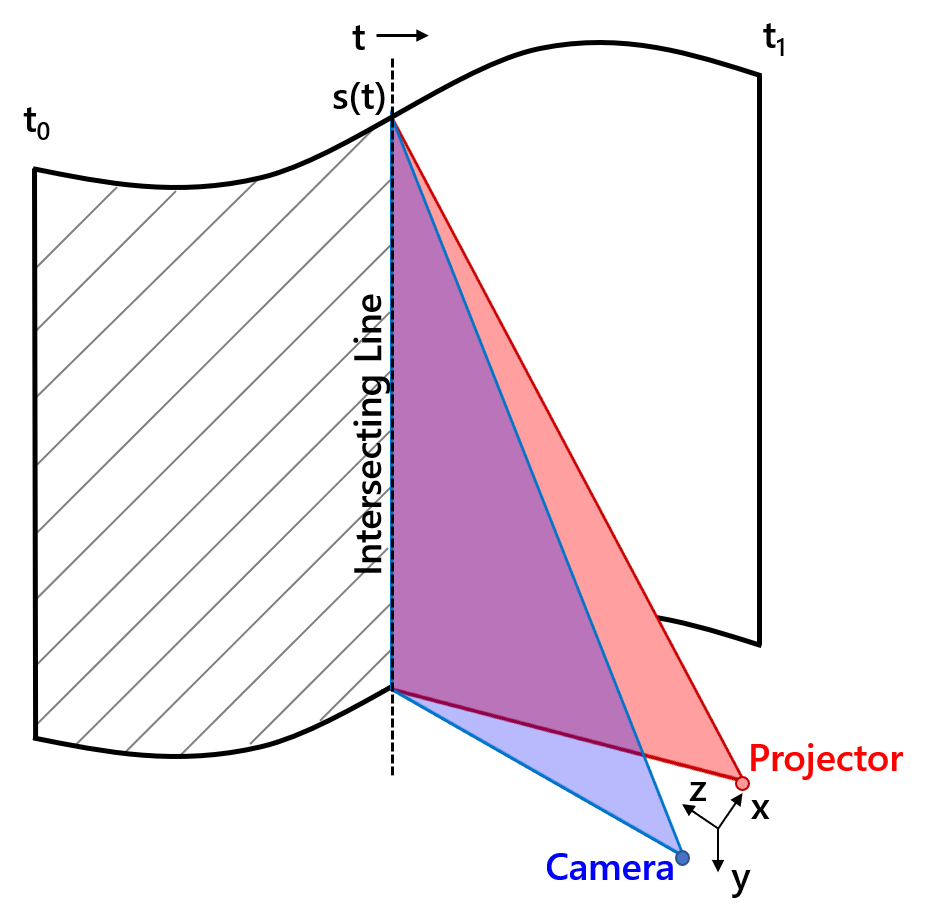
\includegraphics[width=0.9\textwidth]{light_curtain_iso.png} % second figure itself
   % \end{minipage}
   \centering
   \caption{ \textbf{Below:}  The Programmable Light Curtain (LC) device (Image taken from \cite{bartels2019Agile}), consists of a laser, galvomirror and NIR camera. \textbf{Above:} The light curtain senses a ruled 3D surface extruding from a given top-down 2D curve. Surfaces that fall within the \textit{thickness} of the curtain, result in higher intensity.}
   \label{fig:lcdevice} 
\end{figure}

The Light Curtain device consists of a rolling shutter NIR (Near-Infrared) camera flipped vertically (that images planes in the world per pixel row), a Line Laser module and a Galvomirror (that generates planes of light in the world depending on the angle). The exact sensing location is obtained by intersecting (triangulating) these two planes, and sweeping this laser line creates a 3D ruled surface called a light curtain. Do note that the image and light planes have some divergence, so their intersection results in a volume in space (bounded by purple points in Fig~\ref{fig:lcdevice})  with some \textit{thickness}, where any objects that intersect it result in higher intensities in the NIR image.

\begin{figure}[h]
   \centering
   \begin{minipage}{0.5\textwidth}
       \centering
       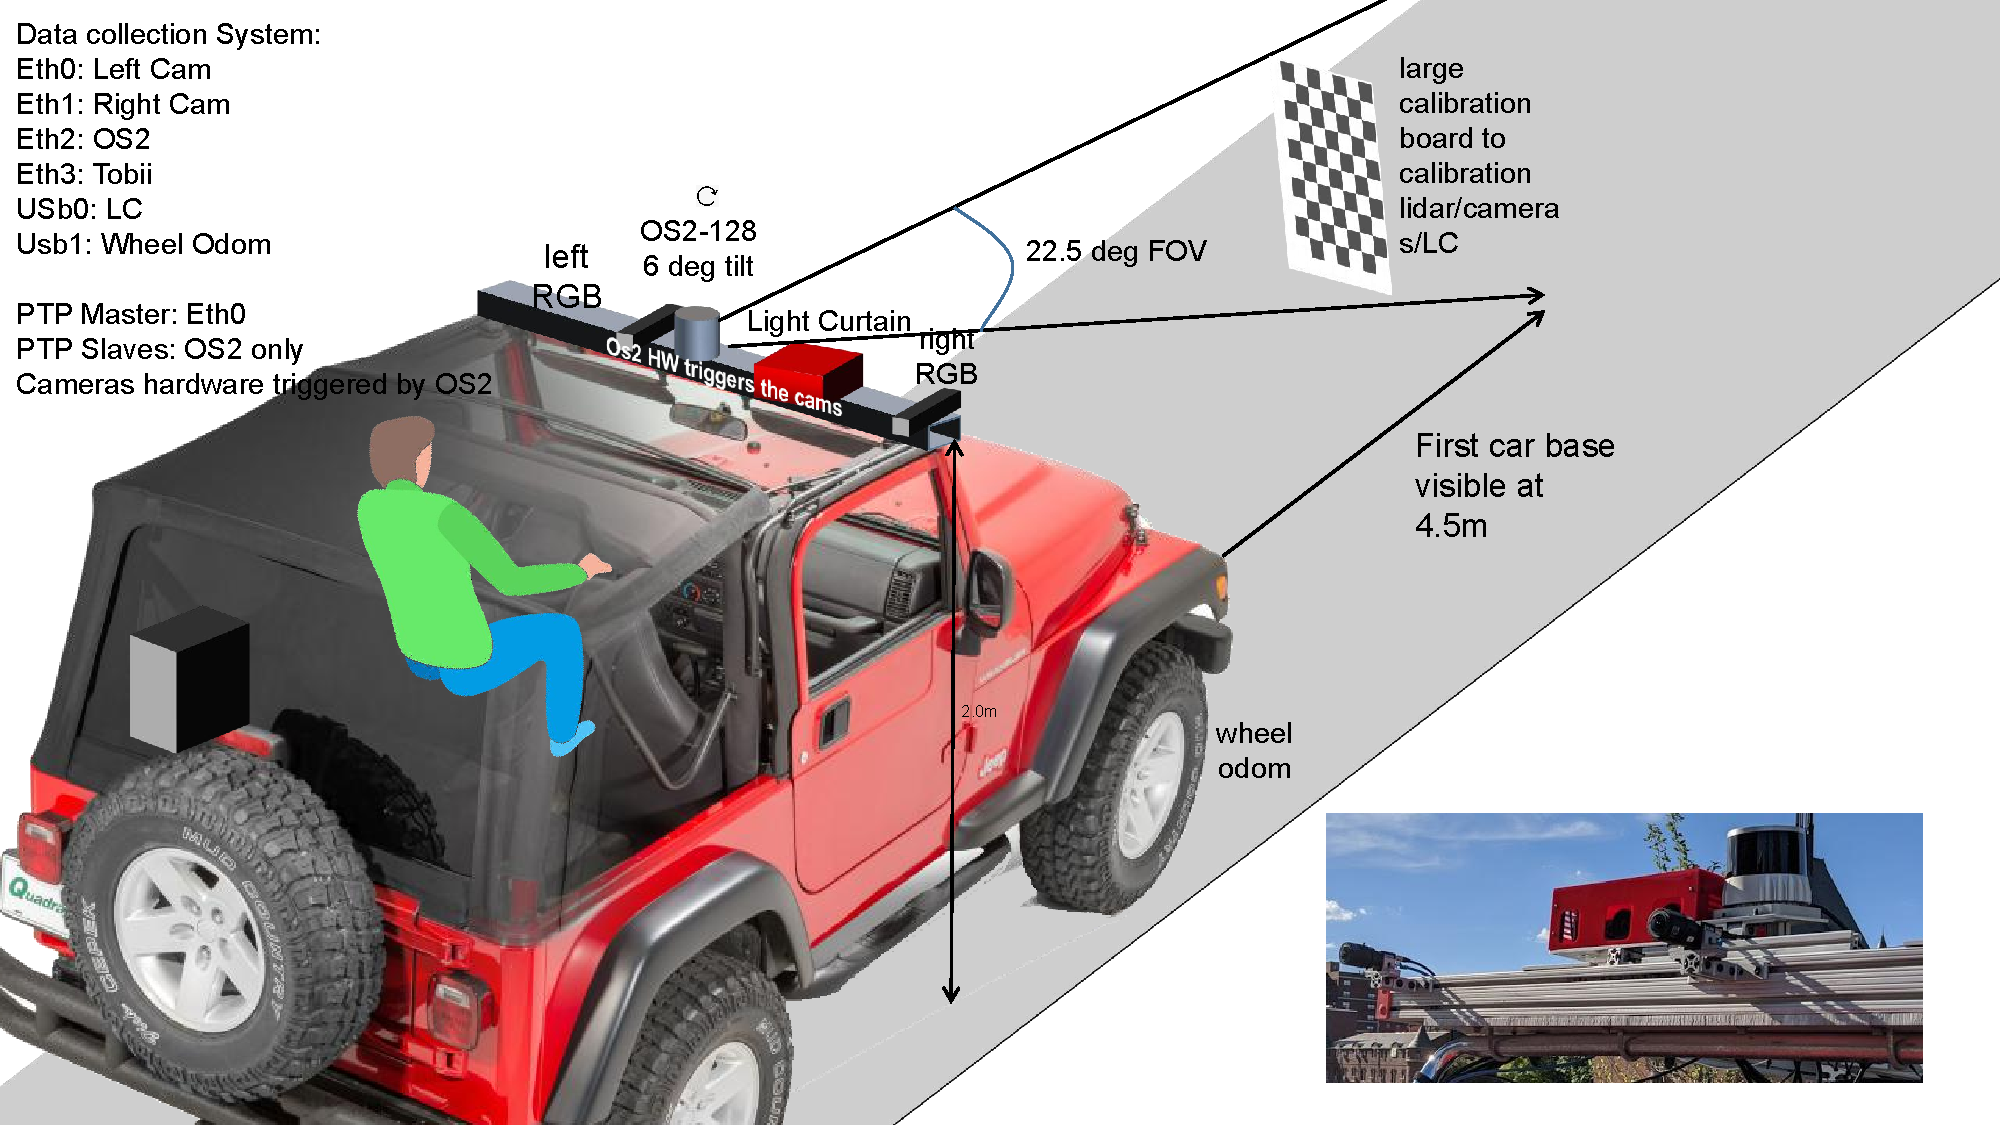
\includegraphics[width=1.0\textwidth]{figures/array.pdf}
   \end{minipage}\hfill
   \centering
   \caption{Setup for real-world experiments: FLIR Stereo camera pair, Light Curtain (LC) and OS2-128 Beam Lidar used for ground truth mounted on a Jeep.}
\end{figure}

To conduct real-world experiments for our algorithms, we setup an array of sensors consisting of a FLIR Stereo Camera Pair with a baseline of 0.7m, Light Curtain device, and an Ouster OS2-128 Lidar for accuracy validation and to assist in training RGB depth estimation networks.

\begin{figure}[h]
   \centering
   \begin{minipage}{0.5\textwidth}
       \centering
       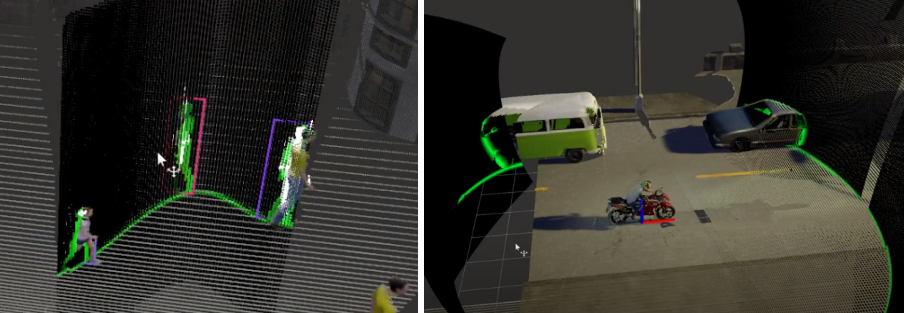
\includegraphics[width=1.0\textwidth]{figures/sim.png}
   \end{minipage}\hfill
   \centering
   \caption{Light Curtain Simulator}
   \label{fig:lcsimkitti} 
\end{figure}
%\vspace{-.1in}
We also designed a Light Curtain Simulator that uses ground truth depth maps to simulate parameters such as NIR instrinsics, Laser extrinsincs, Galvomirror speed, Laser Divergence/Thickness and Laser Angle. This is used in conjunction with the KITTI dataset as seen in Fig~\ref{fig:lcsimkitti}. 

